\chapter{FUNDAMENTAÇÃO TEÓRICA}{}
\label{cap:03}

A bananicultura configura-se como uma das principais atividades agrícolas do Brasil, tanto em termos econômicos quanto sociais, estando presente em todas as regiões do país e sendo praticada por produtores de diferentes escalas. Independentemente do sistema de produção adotado, a adoção de boas práticas agrícolas (BPA) e de boas práticas de fabricação (BPF) é fundamental para garantir a produção de alimentos seguros, ambientalmente responsáveis e economicamente viáveis (EMBRAPA, 2017).
Neste contexto, o presente capítulo tem como objetivo apresentar as principais doenças foliares que afetam a bananeira, detalhando suas causas, sintomas visuais e estágios de desenvolvimento. Essas informações são essenciais para compreender a base visual utilizada na classificação automática por redes neurais convolucionais.

\section{Sigatoka}

A Sigatoka, também conhecida como \textit{doença das manchas nas folhas}, é uma das principais enfermidades que acometem as plantações de bananeira, comprometendo diretamente a fotossíntese e a produtividade das plantas. Esta doença é causada por fungos do gênero \textit{Mycosphaerella}, sendo as duas espécies mais comuns a \textit{Mycosphaerella musicola}, responsável pela \textit{Sigatoka-amarela}, e a \textit{Mycosphaerella fijiensis}, causadora da \textit{Sigatoka-negra} silva2024, embrapa2017\textbf{} \cite{silva2024, embrapa2017}.

Os sintomas da Sigatoka incluem manchas amarelas nas folhas mais velhas, que gradualmente se tornam marrons e necróticas. A progressão da doença leva à morte prematura das folhas, comprometendo a fotossíntese da planta. O controle da doença envolve o uso de fungicidas, práticas culturais como a remoção de folhas infectadas e melhoria da ventilação no dossel da plantação \cite{rezende2020}. A seguir, apresentam-se as duas variantes da doença, com base nas descrições da EMBRAPA \cite{embrapa2017}.

\subsection{Sigatoka-amarela (\textit{Mycosphaerella musicola})}

\subsubsection*{Sintomas}

Os sintomas iniciais aparecem na face superior da folha, como uma leve descoloração em forma de ponto entre as nervuras secundárias da segunda à quarta folha (Figura~\ref{fig:sigatoka_amarela}A). Essas descolorações evoluem para estrias amarelas, que posteriormente tornam-se marrons. Na sequência, surgem manchas necróticas escuras, envoltas por um halo amarelo, com formato elíptico característico (Figura~\ref{fig:sigatoka_amarela}B). Na fase final, o centro da mancha torna-se deprimido, com tecido seco e coloração cinza, circundado por bordos pretos, resultando na necrose de grandes áreas foliares (Figura~\ref{fig:sigatoka_amarela}C).

\begin{figure}[h]
    \centering
    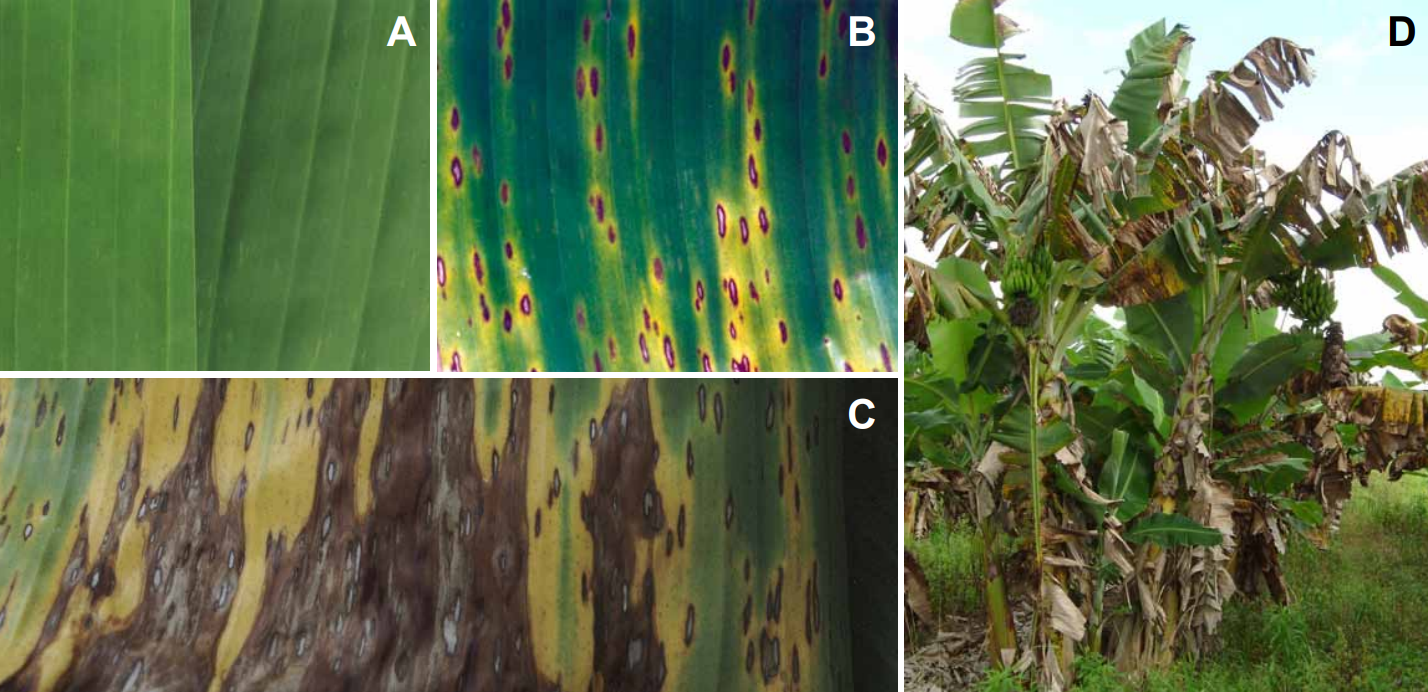
\includegraphics[width=0.9\textwidth]{figuras/capitulo 3/amarela.png}
    \caption{Sintomas da sigatokaamarela: estádios iniciais da doença
(A); manchas elípticas (B); necrose foliar (C); perdas na produção (D).
}
    \label{fig:sigatoka_amarela}
    \small{\textbf{Fonte:} EMBRAPA (2017)}
\end{figure}

\subsubsection*{Estágios de desenvolvimento}

A lesão da Sigatoka-amarela passa por seis estágios principais (Figura~\ref{fig:sigatoka_amarela_estagios}):

\begin{enumerate}
    \item \textbf{Estágio I:} ponto ou risca com até 1 mm de comprimento, com leve descoloração;
    \item \textbf{Estágio II:} estria amarelada com alguns milímetros de comprimento;
    \item \textbf{Estágio III:} estria alargada com coloração vermelho-amarronzada;
    \item \textbf{Estágio IV:} mancha oval alongada, de contornos indefinidos e coloração parda;
    \item \textbf{Estágio V:} presença de halo amarelado e início da esporulação;
    \item \textbf{Estágio VI:} mancha com centro cinza deprimido, bordos pretos e halo amarelo.
\end{enumerate}

\begin{figure}[h]
    \centering
    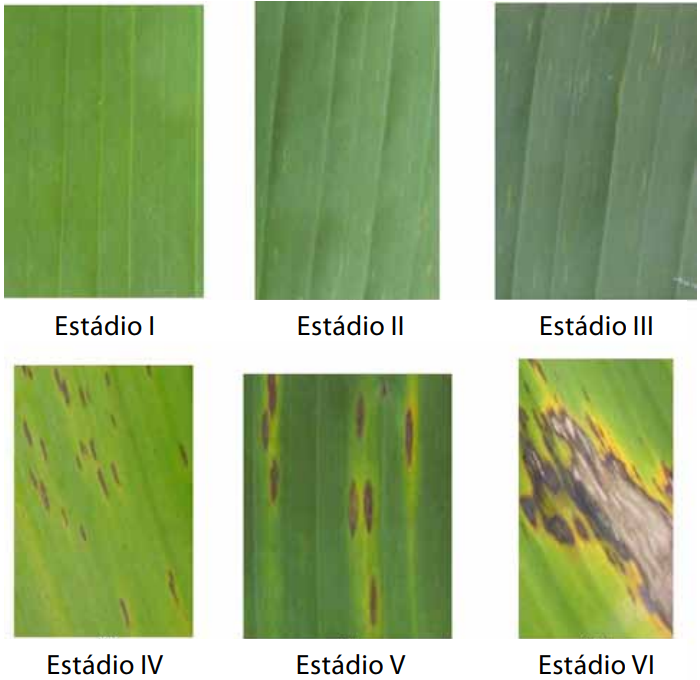
\includegraphics[width=0.7\textwidth]{figuras/capitulo 3/amarela_estagios.png}
    \caption{Estágios de desenvolvimento da lesão de Sigatoka-amarela.}
    \label{fig:sigatoka_amarela_estagios}
    \small{\textbf{Fonte:} EMBRAPA (2017)}
\end{figure}

\subsection{Sigatoka-negra (\textit{Mycosphaerella fijiensis})}

\subsubsection*{Sintomas}

A Sigatoka-negra inicia-se na \textbf{face inferior da folha}, com pontos amarelados que evoluem rapidamente para estrias marrons (Figura~\ref{fig:sigatoka_negra}A, \ref{fig:sigatoka_negra}B). Essas estrias tornam-se negras e visíveis também na face superior (Figura~\ref{fig:sigatoka_negra}C). As estrias, ao coalescerem, formam áreas extensas de necrose, e com frequência não apresentam halo amarelado. Em estágios avançados, observa-se destruição total da folha (Figura~\ref{fig:sigatoka_negra}D).

\begin{figure}[h]
    \centering
    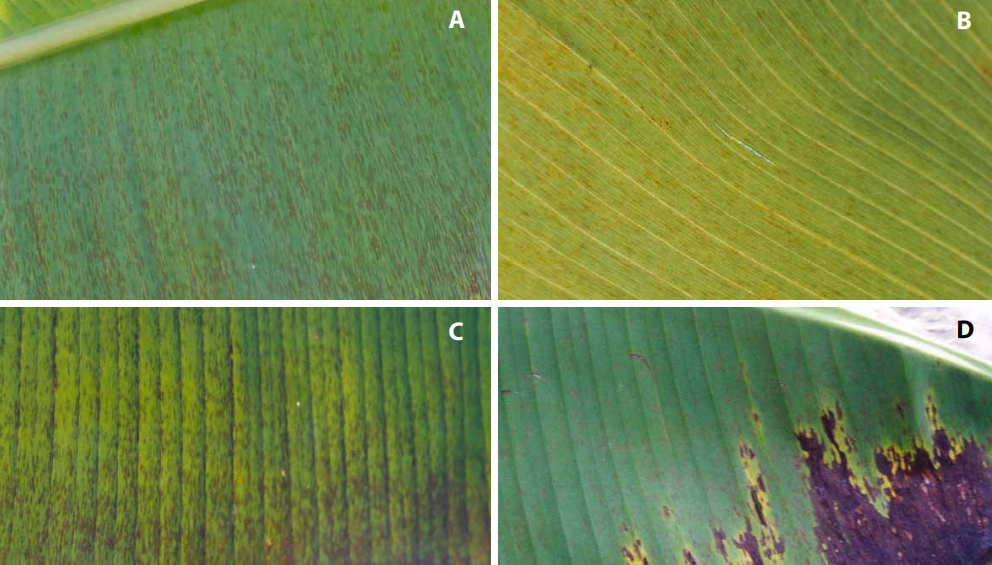
\includegraphics[width=0.7\textwidth]{figuras/capitulo 3/negra.png}
    \caption{Sintomas da Sigatoka-negra: (A, B) estrias marrons na face inferior; (C) necrose na face superior; (D) necrose total.}
    \label{fig:sigatoka_negra}
    \small{\textbf{Fonte:} EMBRAPA (2017)}
\end{figure}

\subsubsection*{Estágios de desenvolvimento}

A lesão da Sigatoka-negra também apresenta seis estágios distintos (Figura~\ref{fig:sigatoka_negra_estagios}):

\begin{enumerate}
    \item \textbf{Estágio I:} pequenos pontos amarelo-amarronzados na face inferior;
    \item \textbf{Estágio II:} estrias marrom-avermelhadas visíveis à luz;
    \item \textbf{Estágio III:} estrias de até 30 mm, quase negras, visíveis em ambas as faces;
    \item \textbf{Estágio IV:} mancha elíptica com halo aquoso marrom-claro;
    \item \textbf{Estágio V:} centro necrótico negro, levemente deprimido, com halo amarelado;
    \item \textbf{Estágio VI:} centro cinza com presença de pseudotécios (pontos negros de esporos).
\end{enumerate}

\begin{figure}[h]
    \centering
    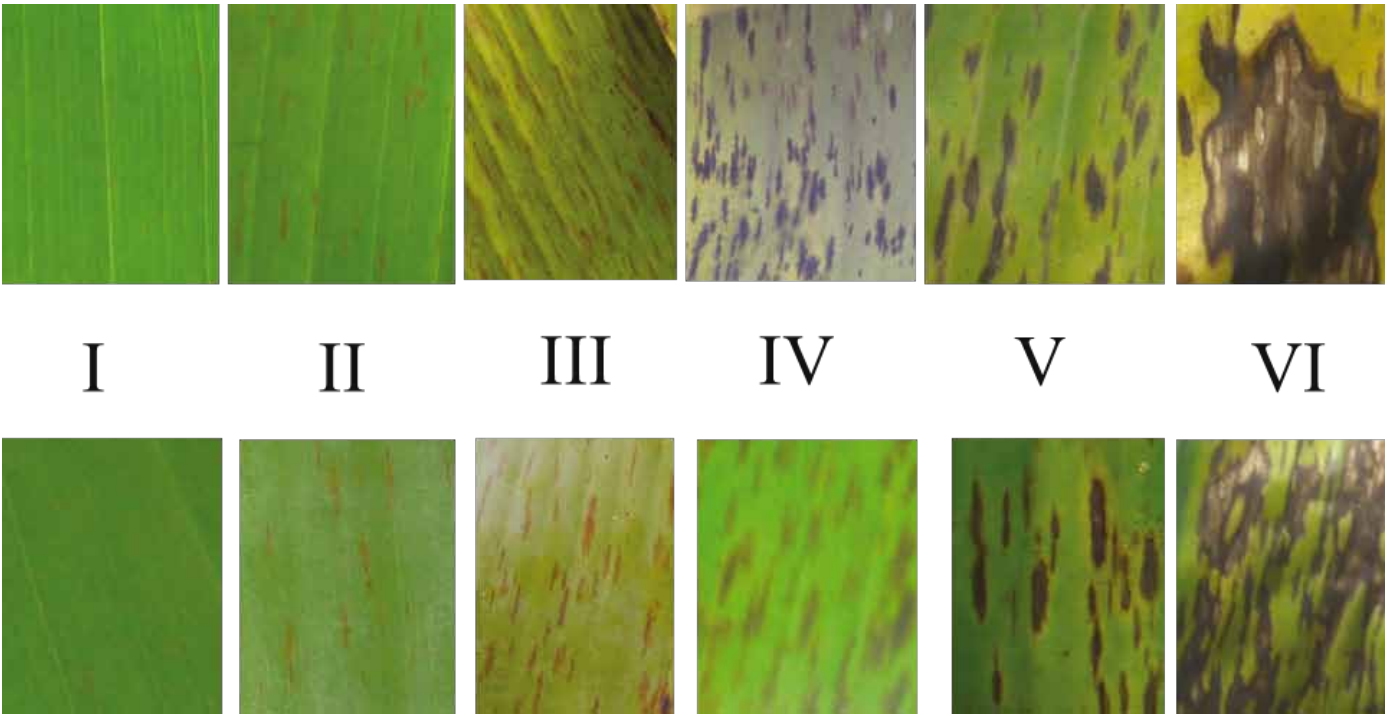
\includegraphics[width=0.8\textwidth]{figuras/capitulo 3/estagios da doenca.png}
    \caption{Estágios de desenvolvimento da lesão de Sigatoka-negra.}
    \label{fig:sigatoka_negra_estagios}
    \small{\textbf{Fonte:} EMBRAPA (2017)}
\end{figure}

\vspace{1em}
A presença de sintomas visuais progressivos e relativamente padronizados, como os apresentados pela Sigatoka-amarela e Sigatoka-negra, fundamenta a proposta de aplicação de redes neurais convolucionais (CNNs) para sua classificação automática por meio de imagens digitais.



\section{Mancha de Cordana (\textit{Neocordana musae})}

A mancha de Cordana é uma doença foliar causada pelo fungo \textit{Neocordana musae} (anteriormente conhecido como \textit{Cordana musae}), que afeta as folhas da bananeira e pode reduzir a capacidade fotossintética da planta, comprometendo a produtividade e a qualidade da produção. Embora seja considerada uma doença secundária em relação à Sigatoka, sua presença está associada ao enfraquecimento do tecido foliar e à umidade excessiva. Em muitos casos, suas lesões evoluem a partir de áreas previamente afetadas por Sigatoka, agravando o estado sanitário das folhas \cite{embrapa2017, pereira2020}.

\subsubsection*{Sintomas}

Os sintomas iniciais da mancha de Cordana podem ser confundidos com os da Sigatoka-amarela. As lesões iniciais apresentam coloração semelhante e formato elíptico, dificultando o diagnóstico visual (Figura~\ref{fig:cordana}A). À medida que evoluem, tornam-se maiores do que o habitual, embora mantenham um padrão visual similar ao das manchas de Sigatoka. Nas fases finais, as lesões atingem vários centímetros de comprimento e largura, sendo caracterizadas por \textbf{zonas concêntricas bem definidas} e circundadas por um \textbf{halo amarelo} (Figura~\ref{fig:cordana}B e \ref{fig:cordana}C).

\begin{figure}[h]
    \centering
    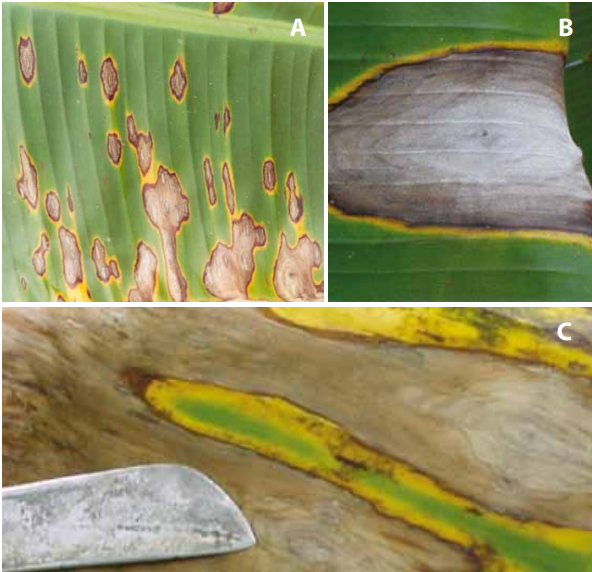
\includegraphics[width=0.5\textwidth]{figuras/capitulo 3/cardana.png}
    \caption{Mancha de Cordana: (A) lesões típicas sobre a folha; (B, C) detalhe das zonas concêntricas características.}
    \label{fig:cordana}
    \small{\textbf{Fonte:} EMBRAPA (2017)}
\end{figure}

A diferenciação entre Cordana e outras doenças foliares é um desafio importante para os produtores e especialistas. A presença de padrões visuais bem definidos, como as zonas concêntricas, contribui para a aplicabilidade de técnicas de visão computacional baseadas em aprendizado profundo, especialmente por redes neurais convolucionais.


\section{Queima foliar por \textit{Pestalotiopsis} (\textit{Pestalotiopsis palmarum})}

A queima foliar causada por \textit{Pestalotiopsis palmarum} é uma doença fúngica comum que afeta diversas espécies de plantas tropicais, incluindo a bananeira. Essa doença compromete diretamente as folhas da planta, resultando em redução da área fotossintética, prejuízo ao crescimento vegetativo e impacto negativo sobre a produção de frutos \cite{pestalotiopsis2020}.

\subsubsection*{Sintomas}

Os primeiros sintomas da infecção por \textit{Pestalotiopsis} incluem \textbf{lesões marrons encharcadas} na superfície das folhas (Figura~\ref{fig:pestalotiopsis}). Essas lesões tendem a se expandir e coalescer, formando áreas maiores de tecido necrosado. Com o avanço da doença, ocorre desfolha precoce e enfraquecimento da planta.

\begin{figure}[h]
    \centering
    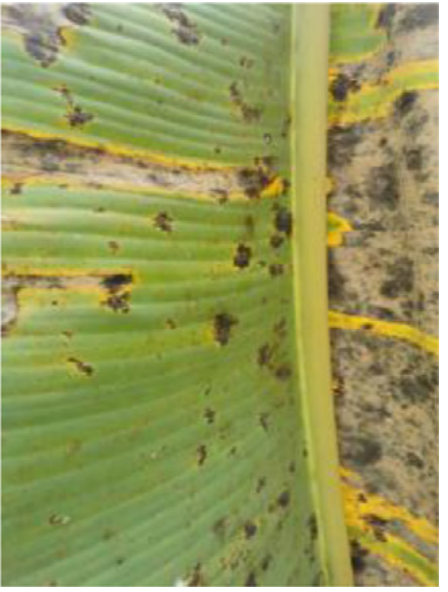
\includegraphics[width=0.5\textwidth]{figuras/capitulo 3/Pestalotiopsis.png}
    \caption{Lesões foliares causadas por \textit{Pestalotiopsis palmarum}: manchas marrons encharcadas em expansão.}
    \label{fig:pestalotiopsis}
    \small{\textbf{Fonte:} Elaborado pelo autor com base em imagens públicas de sintomas da doença.}
\end{figure}

A doença é favorecida por ambientes \textbf{quentes e úmidos}, sendo comum em regiões tropicais. Além disso, pode se espalhar pelo uso de mudas contaminadas ou material vegetativo infectado. A presença de lesões características torna viável o uso de redes neurais convolucionais na detecção automática da doença, uma vez que os padrões visuais são reconhecíveis e recorrentes em imagens foliares.



Apesar da existência de características visuais relativamente padronizadas nas folhas infectadas, a diferenciação precisa entre as doenças foliares da bananeira — como Sigatoka-amarela, Sigatoka-negra, mancha de Cordana e a queima foliar por \textit{Pestalotiopsis} — ainda representa um grande desafio. Isso se deve ao fato de que, especialmente nos estágios iniciais, os sintomas podem apresentar semelhanças visuais significativas. Dessa forma, a identificação correta muitas vezes exige o conhecimento técnico de um especialista ou a realização de exames laboratoriais específicos, o que eleva os custos e torna o processo de diagnóstico inacessível para a maioria dos pequenos e médios produtores rurais.

Cada uma dessas doenças exige estratégias de controle distintas, e um diagnóstico equivocado pode comprometer toda a lavoura, seja por atraso no manejo adequado, seja pela aplicação incorreta de defensivos. Nesse cenário, a aplicação de técnicas computacionais baseadas em aprendizado profundo, como as redes neurais convolucionais (CNNs), surge como uma alternativa promissora. Ao automatizar a classificação das doenças por meio da análise de imagens digitais, essas técnicas possibilitam diagnósticos mais rápidos, acessíveis e com maior precisão, mesmo em regiões onde o acesso a assistência técnica especializada é limitado.



\section{Banco de Dados para Detecção da Doença}


O conjunto de dados adquirido \ac{BananaLSD} possui um banco de imagens divididas em 2 categorias de folhas de bananeira: Sigatoka e saudável. As 2 classes totalizam 530 imagens. Todas as imagens foram rotuladas por um especialista em  patologia de plantas. As imagens foram todas tiradas manualmente com câmeras de smartphone em uma plantação de bananas \cite{DadosArt}. Figura \ref{fig:Fig5} representa as duas características, sendo que, a culuna amarela mostra a quantidade de imagens de sigatoka e a azul a quantidade de imagens saudáveis.  

\begin{figure}[!h]
	\centering
	\caption{Conjunto de dados adquirido \ac{BananaLSD}}
	%\vskip 5mm
	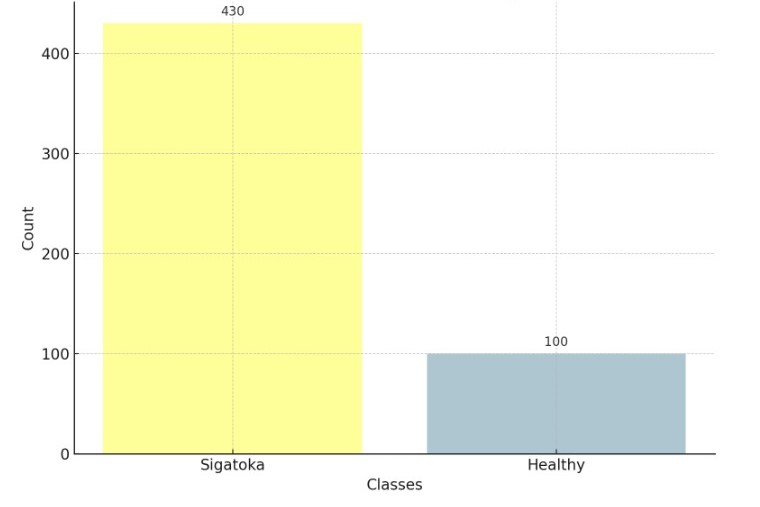
\includegraphics[width=10cm]{figuras/classes Sigatoka e Healthy.jpg}\\
	\autoria{Autoria Própria (2024).}
	\label{fig:Fig5}
\end{figure}

A pasta do conjunto de dados contém duas pastas, uma para o conjunto original e outra para o conjunto aumentado. Ambas essas pastas contêm duas subpastas - sigatoka e saudável - uma para cada uma das classes.


% COMECA AQUI --------------------------------------------------------
\section{Aprendizagem de Máquina e Redes Neurais Artificiais}
\label{sec:aprendizagem-maquina}

% Definindo o ambiente para aprendizagem de máquina
A aprendizagem de máquina é um campo da inteligência artificial que desenvolve algoritmos capazes de aprender padrões a partir de dados, permitindo previsões ou classificações sem programação explícita \cite{mitchell1997machine}. No contexto da bananicultura, a aprendizagem de máquina é aplicada para identificar doenças foliares, como Sigatoka, mancha de Cordana e Pestalotiopsis, a partir de imagens digitais, otimizando o diagnóstico e reduzindo perdas agrícolas \cite{RezendeTese}, \cite{DadosArt}.

O aprendizado supervisionado, foco deste trabalho, utiliza dados rotulados (ex.: imagens de folhas associadas a classes de doenças) para treinar modelos que mapeiam entradas (pixels) para saídas (rótulos). O treinamento minimiza uma função de custo por meio de algoritmos como \textit{gradient descent} e \textit{backpropagation} \cite{Rumelhart1986}. A avaliação do desempenho, descrita na Seção \textcolor{red}{\ref{sec:metodologia}}, utiliza métricas como acurácia (\(Ac\)) e matriz de confusão, definidas pelas Equações \ref{eq:acuracia} e \ref{eq:erro}:

\begin{equation}
Ac = \frac{\sum_{i=1}^m n_{i,i}}{\sum_{i=1}^m \sum_{j=1}^m n_{i,j}}
\label{eq:acuracia}
\end{equation}

\begin{equation}
Cf = 1 - Ac
\label{eq:erro}
\end{equation}

\subsection{Redes Neurais Artificiais}
\label{subsec:rna}

% Definindo o ambiente para RNAs
As redes neurais artificiais (RNAs) são modelos computacionais inspirados no cérebro humano, compostos por neurônios artificiais interconectados que processam informações para realizar tarefas como classificação \cite{Haykin2001}. Uma RNA é formada por camadas de entrada, ocultas e saída, com conexões ponderadas por pesos ajustados durante o treinamento \cite{RezendeTese}.

A Figura \ref{fig:neuron} ilustra um neurônio artificial, que combina entradas \(x_i\) com pesos \(w_i\), adiciona um \textit{bias} \(b\), e aplica uma função de ativação \(f\) (ex.: ReLU) para gerar a saída \(y\):

\begin{equation}
y = f\left(\sum_{i=1}^n w_i x_i + b\right)
\label{eq:neuron}
\end{equation}

\begin{figure}[h]
    \centering
    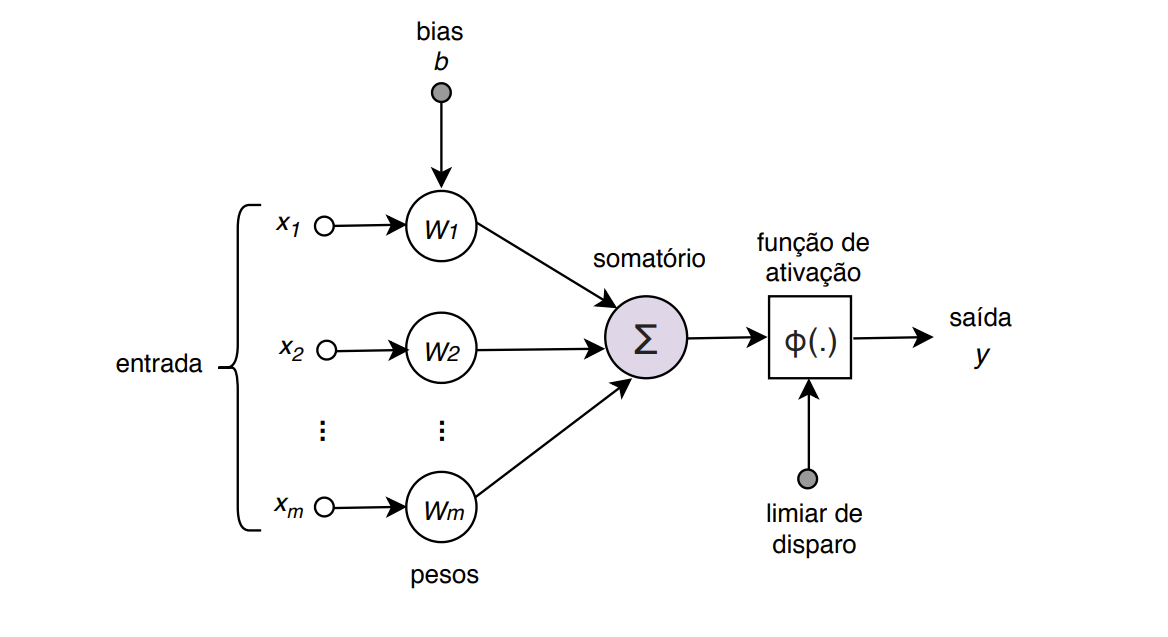
\includegraphics[width=0.8\textwidth]{figuras/NeuronioArtificial.png}
    \caption{Estrutura de um neurônio artificial, com entradas \(x_i\), pesos \(w_i\), \textit{bias} \(b\), e função de ativação \(f\) gerando a saída \(y\).} 
    Adaptado de \cite{RezendeTese}.
    \label{fig:neuron}
\end{figure}








RNAs são eficazes para modelar relações não lineares, sendo amplamente utilizadas em tarefas de reconhecimento de padrões, como a identificação de doenças em plantas \cite{Goodfellow2016}. No entanto, para imagens, as RNAs tradicionais são limitadas, exigindo arquiteturas especializadas como as redes neurais convolucionais (CNNs) \cite{leite2022}.

\section{Redes Neurais Convolucionais}
\label{sec:cnns}

% Definindo o ambiente para CNNs
As redes neurais convolucionais (CNNs) são projetadas para processar dados estruturados, como imagens, utilizando operações de \textit{convolução} para extrair características locais (ex.: bordas, texturas) \cite{LeCun1998}. No contexto deste trabalho, as CNNs são aplicadas para classificar imagens do conjunto BananaLSD, identificando padrões visuais de doenças como Sigatoka, Cordana e Pestalotiopsis \cite{DadosArt}.

\subsection{Estrutura de uma CNN}
\label{subsec:estrutura-cnn}

% Definindo a estrutura geral de uma CNN
Uma CNN é composta por:

\begin{itemize}
    \item \textbf{Camadas de Convolução}: Aplicam filtros (\textit{kernels}) para gerar mapas de características, destacando padrões como manchas ou estrias em folhas. A Figura \ref{fig:convolution} ilustra a operação de convolução.
    \item \textbf{Camadas de \textit{Pooling}}: Reduzem a dimensionalidade espacial (ex.: \textit{max pooling}), aumentando a invariância a transformações \cite{Goodfellow2016}.
    \item \textbf{Camadas Totalmente Conectadas}: Combinam características para a classificação final (ex.: saudável ou doente) \cite{RezendeTese}.
    \item \textbf{Funções de Ativação}: Introduzem não linearidades (ex.: ReLU) para modelar relações complexas \cite{Krizhevsky2012}.
\end{itemize}



A Figura \ref{fig:cnn} apresenta a arquitetura geral de uma CNN, com camadas de convolução, \textit{pooling} e totalmente conectadas, utilizada para classificar doenças em bananeiras.

\begin{figure}[h]
    \centering
    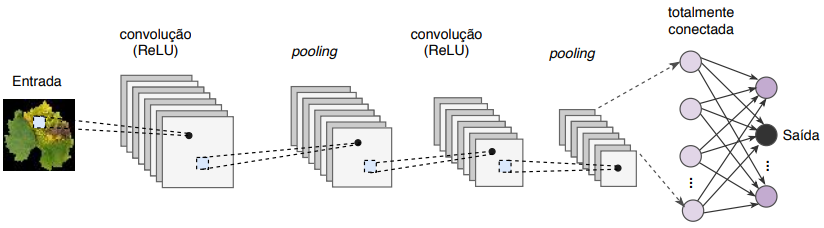
\includegraphics[width=0.9\textwidth]{figuras/capitulo 3/cnn.png}
    \caption{Arquitetura de uma CNN, processando imagens de folhas para classificar doenças. Adaptado de \cite{RezendeTese}.}
    \label{fig:cnn}
\end{figure}



\begin{figure}[h]
    \centering
    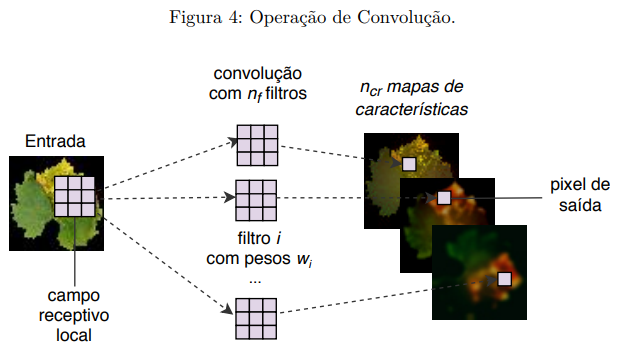
\includegraphics[width=0.8\textwidth]{figuras/capitulo 3/convolution_process.png}
    \caption{Operação de convolução, onde um filtro é aplicado a uma imagem para gerar um mapa de características. Adaptado de \cite{RezendeTese}.}
    \label{fig:convolution}
\end{figure}








%INICIO--------------------------------------------------------------------------------------------------------------------



\subsection{Arquitetura AlexNet}
\label{subsec:alexnet}

A AlexNet, proposta por \cite{Krizhevsky2012}, representou um marco no aprendizado profundo ao vencer o desafio ImageNet Large Scale Visual Recognition Challenge (ILSVRC) de 2012, destacando-se pela eficácia das redes neurais convolucionais (CNNs) em tarefas de classificação de imagens. Com aproximadamente 61 milhões de parâmetros, a AlexNet estabeleceu um novo padrão para arquiteturas de visão computacional \cite{Krizhevsky2012}.

A arquitetura da AlexNet é composta por oito camadas principais: cinco camadas convolucionais seguidas por três camadas totalmente conectadas, conforme ilustrado na Figura \ref{fig:alexnet}. As camadas convolucionais 1, 2 e 5 são seguidas por operações de \textit{max pooling}, que reduzem a dimensionalidade espacial e aumentam a invariância a transformações locais \cite{Goodfellow2016}. As camadas convolucionais 3 e 4 são diretamente conectadas, sem operações intermediárias. A camada final utiliza a função de ativação \texttt{softmax} com 1000 unidades, correspondendo às classes do desafio ImageNet \cite{Krizhevsky2012}.

A função de ativação ReLU (\(f(x) = \max(0, x)\)) é aplicada nas primeiras sete camadas, acelerando o treinamento ao introduzir não linearidades e mitigando o problema do desaparecimento do gradiente em comparação com funções como \textit{sigmoid} \cite{Braga2024}. Para reduzir o \textit{overfitting}, a AlexNet emprega \textit{dropout} com probabilidade de 50\% nas duas primeiras camadas totalmente conectadas, desativando neurônios aleatoriamente durante o treinamento para melhorar a generalização \cite{Hinton2012}. Além disso, utiliza \textit{overlapping pooling} com janelas de 3x3 e \textit{stride} de 2, permitindo maior captura de características espaciais em comparação com \textit{pooling} tradicional \cite{Krizhevsky2012}.

\begin{figure}
    \centering
    \includegraphics[width=0.9\textwidth]{images/alexnet_architecture.png}
    \caption{Arquitetura simplificada da AlexNet, com cinco camadas convolucionais, \textit{max pooling} e três camadas totalmente conectadas. Fonte: autoria própria (2024).}
    \label{fig:alexnet}
\end{figure}

A AlexNet também implementa aumento de dados (\textit{data augmentation}), como translações e espelhamentos horizontais, para enriquecer o conjunto de treinamento. Uma inovação significativa foi o uso de duas GPUs em paralelo, dividindo as camadas convolucionais em dois caminhos para acelerar o treinamento \cite{Krizhevsky2012}. Essas características, combinadas com sua profundidade, tornaram a AlexNet uma referência em arquiteturas de CNNs.


%fim alex nbet--------------------------------------------------------------------------------------------------------------------


























\subsection{Vantagens das CNNs na Bananicultura}
\label{subsec:vantagens-cnns}

% Definindo as vantagens das CNNs
As CNNs oferecem benefícios para a classificação de doenças foliares \cite{LeCun2015}:

- **Extração Automática de Características**: Aprendem padrões diretamente dos pixels, eliminando a necessidade de \textit{feature engineering} manual \cite{RezendeTese}.
- **Invariância Espacial**: Operações de \textit{pooling} permitem reconhecer sintomas independentemente de sua posição na imagem \cite{Goodfellow2016}.
- **Robustez**: Técnicas como ampliação de dados (ex.: rotação, ajuste de brilho) aumentam a generalização, como descrito na Seção \ref{sec:metodologia} \cite{Leite2022}.

No presente trabalho, as CNNs (ex.: AlexNet, ResNet-32) classificam imagens do BananaLSD, apoiando o diagnóstico precoce em regiões como Bom Jesus da Lapa \cite{Silva2024}.


